\documentclass[12pt]{article}

\usepackage{amsmath}
\usepackage{enumitem}
\usepackage{hyperref}
\usepackage[utf8]{inputenc}
\usepackage{graphicx}
\usepackage{rotating}

\usepackage{geometry}
%for 0.75" margins
\geometry{textheight=9.5in, textwidth=7in}
%for 1" margins
%\geometry{textheight=9in, textwidth=6.5in}

\title{CS 450 Final Project Report}
\author{Sean Rettig}
\begin{document} 

\maketitle

\section{Original Proposal}

\subsection{"Yet Another Minecraft Clone"}

I imagine that you'll probably get a dozen or so of these, but it's something that I want to do!
The project would basically be implementing a basic version of the video game Minecraft that includes:
\begin{itemize}
    \item A 3D world filled with textured blocks that is automatically generated
\item At least 5 block types, including:
    \begin{itemize}
        \item At least one non-cube block
        \item At least one block that emits light
        \item At least one block with different textures on each side
        \item At least one block that is partially transparent
    \end{itemize}
    \item Lighting, including from the sun and from light blocks
    \item At least one animal model (with animation and motion)
    \item A player that is controlled by the user to move around and look at the world
    \item The ability to place and destroy blocks
    \item A third-person view for the player
    \item A first-person view for the player that shows the player's hand, plus animation
\end{itemize}

\subsection{Mike Bailey's Comments}

Sean --

Your FP looks fine, but I think it's too much.  The blocks don't have to be textured.  Stick with cubes.  Don't worry about the hand.

-- PB

\section{Modified Proposal}

\subsection{"Yet Another Minecraft Clone"}

I imagine that you'll probably get a dozen or so of these, but it's something that I want to do! 
The project would basically be implementing a basic version of the video game Minecraft that includes:
\begin{itemize}
    \item A 3D world filled with colored blocks that is automatically generated
    \item At least 5 block types, including:
    \begin{itemize}
        \item At least one block that emits light
        \item At least one block that is partially transparent
    \end{itemize}
    \item Lighting, including from the sun and from light blocks
    \item At least one animal model (with animation and motion)
    \item A player that is controlled by the user to move around and look at the world
    \item The ability to place and destroy blocks
    \item A third-person view for the player
    \item A first-person view for the player
\end{itemize}

\section{Report}

For my final project, I ended up implementing everything in the modified
proposal.  The 3D world is generated procedurally, placing layers of stone and
dirt for the base, and using various functions and sine waves to place the
grassy hills on top.  I also manually placed a few light blocks of different
types and a partially transparent block just to show the different types of
blocks available.  These types of blocks can also be placed by the player by
pressing the 'n' or 'm' keys, or broken using the ',' key.  The location that
will be affected is approximately 2 blocks in front of the player and is
indicated by a wireframe cube.  The player can move around the world using the
WASD keys, can move up using the spacebar, and can move down with 'q'.  The
player can also change the direction they are looking by clicking and dragging
across the screen with the mouse, just like in the other demos.

In order to simplify the program a bit and make it fit my mental model, I also
rewrote it such that rather than transforming everything in the world to change
your point of view, the world geometry is static and it is the camera that
moves around, fixed to the player's position.  This also made making the
third-person mode easier, as the view is simply backed up to behind the player
rather than staying at the player's head.  The viewing mode can be toggled with
the 'v' key.

In addition, there is a sun high above the world and a small blue "bird" that
has been animated to fly around above the map in a giant loop.

Overall, my project didn't really deviate from the proposal.  I did, however,
learn a lot, including how to actually implement transparency.  I also had to
do a big trigonometry refresher in order to rewrite the program's camera model
(since the camera actually moves around the scene now) and get the block the
player is looking at (for breaking and placing blocks, as well as showing the
selection outline), among other things.  In order to get the camera to look at
the correct position, I basically had to try and always make the camera focus
on a point just in front of the player, since I couldn't just specify a
direction to look in.  One other particularly interesting thing I learned is
how to dynamically create lights.  Since the player can create and destroy
light blocks, and in any order, I had to create a system that would keep track
of which OpenGL light IDs (e.g. GL\_LIGHT0, GL\_LIGHT1, etc.) were available
for use.  Whenever a light block is placed, the program searches an array of
lights until it finds one that is available, and uses that.  Whenever a block
is destroyed, it removes that light from the array so that it can be reused
later.

\pagebreak

First person view, showing the world, the sun, the bird (in the background on
the right), some red and white light blocks, a transparent block, and the
selection outline:

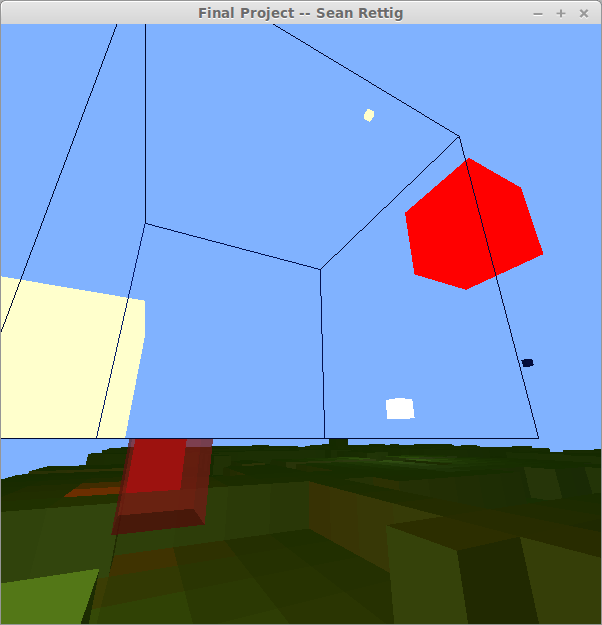
\includegraphics[width=0.55\textwidth]{screenshot1.png}

Third person view, showing the edge of the world, additional blocks, and the
back of the player model (which is also slightly transparent so you can still
see what's in front of you):

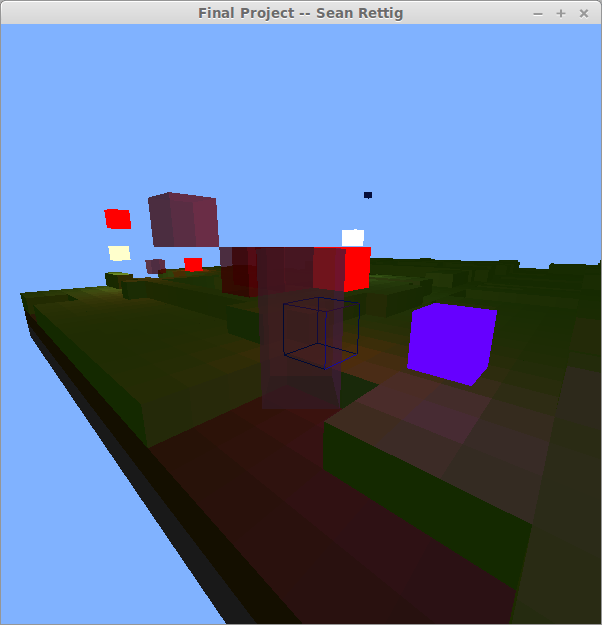
\includegraphics[width=0.55\textwidth]{screenshot2.png}

\end{document}
